\documentclass[11.5pt]{sig-alternate} % sets document style to sig-alternate
% packages
% typesetting
%\usepackage{dirtytalk} % typset quotations easier (\say{stuff})
\usepackage{hanging} % hanging paragraphs
\usepackage[defaultlines=3,all]{nowidow} % avoid widows
\usepackage[pdfpagelabels=false]{hyperref} % produce hypertext links, includes backref and nameref
\usepackage{xurl} % defines url linebreaks, loads url package
\usepackage{microtype}
%\usepackage[super]{nth} % easily create superscript ordinal numbers with \nth{x}
\usepackage{textcomp}
\newcommand{\texttildemid}{\raisebox{0.4ex}{\texttildelow}}
\usepackage{fontspec}
\usepackage{amssymb}
% layout
%\usepackage{enumitem} % control layout of itemize, enumerate, description
\usepackage{fancyhdr} % control page headers and footers
\usepackage{float} % improved interface for floating objects
%\usepackage{multicol} % intermix single and multiple column pages
% language
\usepackage[utf8x]{inputenc} % accept different input encodings
\usepackage[english]{babel} % multilanguage support
\usepackage{braille}
% misc
\usepackage{graphicx} % builds upon graphics package, \includegraphics
%\usepackage{lastpage} % reference number of pages
%\usepackage{comment} % exclude portions of text (?)
\usepackage{xcolor} % color extensions
\usepackage[backend=biber, style=apa]{biblatex} % sophisticated bibliographies % necessary for HTML to display author info and date on abstract page
\usepackage{csquotes} % advanced quotations, makes biblatex happy
\usepackage{authblk} % support for footnote style author/affiliation
% tables and figures
\usepackage{tabularray}
%\usepackage{array} % extend array and tabular environments
\usepackage{caption} % customize captions in figures and tables (rotating captions, sideways captions, etc)
%\usepackage{cuted} % allow mixing of \onecolumn and \twocolumn on same page
\usepackage{multirow} % create tabular cells spanning multiple rows
%\usepackage{subfigure} % deprecated, support for manipulation of small figures
%\usepackage{tabularx} % extension of tabular with column designator "x", creates paragraph-like column whose width automatically expands
%\usepackage{wrapfig} % allows figures or tables to have text wrapped around them
%\usepackage{booktabs} % better rules
% dummy text
%\usepackage{blindtext} % blind text dummy text
%\usepackage{kantlipsum} % Kant style dummy text
\usepackage{lipsum} %lorem ipsum dummy text
% other helpful packages may be booktabs, longtable, longtabu, microtype
\pagestyle{fancy} % sets pagestyle to fancy for fancy headers and footers

% header and footer
% modern way to set header image
\renewcommand{\headrulewidth}{0pt} % defines thickness of line under header
\renewcommand{\footrulewidth}{0pt} % defines thickness of line above header
\setlength\headheight{80.0pt} % sets height between top margin and header image, effectively moves page contents down
\addtolength{\textheight}{-80.0pt} % seems to affect the lower height. maybe only works properly if footer numbers enabled?
\fancyhf{}
\fancyhead[CE, CO]{
\includegraphics[width=\textwidth]{headerImage.png}}
% footer
%\fancyfoot[LE,LO]{Article Title Here \\ DOI: }% left footer article title and doi
%\fancyfoot[CE,CO]{{}} % center footer empty
%\fancyfoot[RE,RO]{\thepage} % right footer page numbers
%\pagenumbering{arabic} % arabic (1, 2, 3) numbering in footer

\hypersetup{colorlinks=true,urlcolor=blue} % sets link color to blue
\urlstyle{same} % sets url typeface to same as rest of text

% set caption and figure to italics, label bold, left align captions, does not transfer to HTML
\captionsetup{labelfont=bf, font={large, it}, justification=raggedright, singlelinecheck=false}
\renewcommand\theContinuedFloat{\alph{ContinuedFloat}}

%this next bit is confusing, but essentially changes the width of the abstract. Seems to have been copied from this https://tex.stackexchange.com/questions/151583/how-to-adjust-the-width-of-abstract
\let\oldabstract\abstract
\let\oldendabstract\endabstract
\makeatletter %changes @ catcode to enable modification (in parsep)
\renewenvironment{abstract} %alters the abstract environment
{\renewenvironment{quotation}%
               {\list{}{\addtolength{\leftmargin}{1em} % change this value to add or remove length to the the default ?
                        \listparindent 1.5em%
                        \itemindent    \listparindent%
                        \rightmargin   \leftmargin%
                        \parsep        \z@ \@plus\p@}%
                \item\relax}%
               {\endlist}%
\oldabstract}
{\oldendabstract}
\makeatother %changes @ catcode to disable modification

% checks
% italics -
% links -
% dashes -
% tildes -
% dollars -
\begin{document}

\title{A direct TeX-to-Braille transcribing method}

\author[1]{\large \color{blue}Andreas Papasalouros}
\author[1]{\large \color{blue}Antonis Tsolomitis}
\affil[1]{University of the Aegean}

\toappear{}
%% ABSTRACT
\maketitle
\begin{@twocolumnfalse} 
\begin{abstract}
\item 
\textit{The TeX/LaTeX typesetting system is the most wide-spread system for creating documents in Mathematics and Science. However, no reliable tool exists to this day for automatically transcribing documents from the above formats into Braille/Nemeth code. Thus, visually impaired students of related fields do not have access to the bulk of study material available in LaTeX format. We have developed a tool, named latex2nemeth, for directly transcribing LaTeX documents to Nemeth Braille, thus facilitating the access of blind students to Science. In order to support the extensive set of Mathematics symbols covered by TeX, we propose some new symbols based on the extension mechanisms of the Nemeth code.}
\\ \\
Keywords: visually impaired, Mathematics Education, content accessibility
\end{abstract}
\end{@twocolumnfalse}

%% AUTHOR INFORMATION

\textbf{*Corresponding Author, Andreas Papasalouros}\\
\href{mailto: andpapas@aegean.gr}{(andpapas@aegean.gr)} \\
\textit{Submitted Dec 14 2016 }\\
\textit{Accepted Apr 25 2017} \\
\textit{Published online Aug 28 2017} \\
\textit{DOI:10.14448/jsesd.08.0003} \\
\pagebreak
\clearpage

\begin{large}
\section*{INTRODUCTION}

Students with disabilities are underrepresented in STEM (Science Technology and Mathematics) fields (Isaacson \& Michaels, 2015). Inadequate access to specialized content, in the form of scientific documents is likely to discourage students with blindness or low vision (BLV) from studying and pursuing STEM careers.  Several studies indicate that this discrepancy can be reduced by “the development and provision of tools for increasing information accessibility” (eg, Isaacson, Schleppenbach, \& Lloyd, 2010/11).  

It is a fact that the great majority of scientific documents (and not only those) are composed in TeX and its derivatives. TeX (from the Greek word "$\tau \acute{\varepsilon} \chi \nu \eta$", meaning, Art) provides a specialized markup language, a form of text files enriched with appropriate commands for supporting typography, eg spacing, indentation, fonts, etc. It was invented by the computer scientist and mathematician Donald Knuth as a technology for producing high quality mathematical printed documents, books, papers, lecture notes, etc. Thus, TeX and its derivatives (LaTeX, XeLaTeX, etc) define a specialized formalism for describing mathematical expressions. Authors and content providers create, through direct typing or by using specialized authoring environments, enhanced text documents in TeX format. The TeX system also comprises a suite of software tools that translate the initial TeX documents into a printable form such as Post\-script and PDF, ready to be printed in traditional and digital facilities.
 
TeX and its derivatives are the standard for writing Mathematics as it can be easily seen by checking the main publication houses of Mathematical literature, such as the American Mathematical Society\footnote{\url{http://www.ams.org/publications/authors/authors}},  SpringerVerlag\footnote{\url{https://www.springer.com/gp/authors-editors/book-authors-editors/manuscript-preparation/5636}},  Elsevier\footnote{\url{https://www.elsevier.com/authors/book-authors/science-and-technology-book-publishing/things-to-consider-as-you-prepare-your-manuscript\#Manuscript and https://www.elsevier.com/authors/author-schemas/latex-instructions}},  Wiley and Sons\footnote{\url{https://authorservices.wiley.com/author-resources/book-authors/prepare-your-manuscript/wiley-latex-template.html}}  etc., as well as arXiv\footnote{\url{https://arxiv.org/} and \url{https://arxiv.org/help/submit_tex}},  the main archive of research articles in Mathematics and other sciences.  Moreover, all research in Mathematics is almost exclusively published in TeX and its derivatives as it can be easily seen on all major journal webpages (all journals state that the manuscript should be in TeX/LaTeX and some say that Word files could be accepted, but this is rare). Since the list is extremely long let us mention some of the best journals, such as 

\begin{itemize}
    \item 	Acta Mathematica, only LaTeX or TeX;\footnote{\url{http://www.mittag-leffler.se/publications/acta-mathematica/submission-manuscripts\#main-content}}
    \item 	Inventiones Mathematicae, mainly LaTeX, Word may be acceptable;\footnote{\url{http://www.springer.com/mathematics/journal/222}}
    \item 	Advances in Mathematics, LaTeX for final submission;\footnote{\url{https://www.journals.elsevier.com/advances-in-mathematics}}
    \item 	Annals of Mathematics, only LaTeX;\footnote{\url{http://annals.math.princeton.edu/submission-guidelines}}
    \item 	Bulletin of the American Mathematical Society, only LaTeX and AMSLaTeX for final submission;\footnote{\url{http://www.ams.org/publications/journals/journalsframework/bullsubmit}}
    \item 	Duke Mathematical Journal, only LaTeX;\footnote{\url{https://www.dukeupress.edu/duke-mathematical-journal}}
    \item 	Geometric and Functional Analysis, only LaTeX.\footnote{\url{http://www.springer.com/birkhauser/mathematics/journal/39}}
\end{itemize}

However, although the method of transcribing a scientific document, such as a Mathematics book, has been created by A. Nemeth in the early ’70s, and it has been a well-established standard in many countries, there has not been a direct and complete solution for passing from TeX into Braille/Nemeth. Since TeX is a highly structured language, a fact that facilitates the translation to Braille, it was a surprise for us to see that relative tools do not exist. Partial solutions exist, however they are not adequate for a reliable translation from TeX/LaTeX into Braille. 

STEM educational and scientific content is currently translated into Braille/Nemeth mainly from MS Word sources that are transcribed by using tools such as (Duxbury Systems, n.d.). The output is embossed by using specialized Braille embossers. However, as mentioned earlier, most scientific content in Mathematics is available in TeX instead of Word format. Furthermore, the translation from TeX into Braille/Nemeth can be performed by initially converting TeX documents into Word or various intermediate formats, and then into Braille. However, this process is unreliable, producing errors and omissions of expressions from the original documents.

Several tools exist for translating mathematical documents from TeX and other mathematics formats into Braille/Nemeth form. A non-exhaustive list could contain Duxbury (Duxbury Systems, n.d.), UMA (Karshmer et al., 2004), UMCL (Archambault et al., 2005), MAVIS (A. Karshmer, Gupta, Geiger, \& Weaver, 1999), MathBraille (Hara et al., 2000) and Blind Friend\-ly LaTeX (Gonzúrová \& Hrabák, 2012). Also, certain configurations of tools have been used to translate from TeX to Braille/Nemeth by using intermediate formats such as RTF (Rich Text Format) and MathML (Mathematical Markup Language) (W3C, 2003). For example, the text4\-ht software (Gurari, 2004) translates TeX to MathML and then the liblouis project (Egli, 2011) can be used for producing Braille from MathML.  However, although these tools and configurations are reported to translate from TeX to Nemeth, we were not able to successfully use them in order to produce mathematical documents of the complexity required in University level Mathematics and Science. The latex2nemeth tool, presented in this paper, aims at the reliable transcription of available books and course notes, intending to support the development of a repository for Mathematical texts for blind students and researchers. To the best of our knowledge, none of the existing systems has \textit{demonstrably} fulfilled these goals.

In this paper, we propose a method for transcribing Mathematics documents from TeX/La\-TeX and its derivatives directly into Braille. This transcription should satisfy the following requirements: a) Correct transcription, containing no errors, b) support for extended sets of mathematical symbols, such as the ones used in scientific books and text books, c) minimum intervention of a human user, and c) support for images that are also expressed in appropriate LaTeX libraries. A software tool has been developed for automating this transcription satisfying the above requirements. Given that the Mathematics symbol set of TeX is extensive, several of its symbols are not supported by the Nemeth code. Thus, we also propose some new extensions to the Nemeth code so as to encode TeX symbols not supported in Braille by using the Nemeth code extension mechanism. We have tested our tools by the transcription of an actual Mathematics book published by AMS, a Greek mathematics textbook that is used as a textbook in a Mathematics department, and several sets of course notes. Furthermore, we have also conducted a quantitative evaluation of the reliability of the tool, which is also presented later.

The structure of this paper is as follows: In the next section we present certain proposed extensions to the Nemeth code in order to widely cover advanced mathematics symbols. Then, the functionality of the proposed system is presented, followed by the description of its implementation. The following section contains a quantitative evaluation, as well as a case study for the evaluation of the proposed tool, and the paper ends with some conclusions and considerations for future work.

\section*{PROPOSED EXTENSIONS TO NEMETH CODE}

The Nemeth Code (Nemeth, 1972), published in 1972, describes rules for unambiguously encoding mathematical expressions using six-dot Braille symbols thus supporting the printing of mathematical/technical documents in a form readable to visually impaired persons. It defines the structure of complex mathematical expressions and contains an extensive list of symbols.

Most importantly, the Nemeth Code provides composition rules, so that new symbols can be created from old ones. For example, by using these rules, for representing hookrightarrow ($\hookrightarrow$), used for denoting subspaces in Mathematical Analysis, a new symbol can be composed in Braille form as \fontspec[Script=Braille]{DejaVu Serif} ⠫⠈⠯⠒⠒⠕ \fontspec{Latin Modern Roman} Table 1 shows a small, indicative list of such composed symbols.

The Nemeth code, in order to represent as many language/ math symbols as possible by using only 64 six-dot braille symbols, reserves some of the six-dot symbols for special purposes. In the previous example, the symbol \fontspec[Script=Braille]{DejaVu Serif} ⠫ \fontspec{Latin Modern Roman} is reserved to mean the beginning of the description of a symbol or picture. And although the symbols that follow \fontspec[Script=Braille]{DejaVu Serif} ⠫ \fontspec{Latin Modern Roman} in the above example may have their own meaning (for example \fontspec[Script=Braille]{DejaVu Serif} ⠕ \fontspec{Latin Modern Roman} is the letter “o”), when they are read after the \fontspec[Script=Braille]{DejaVu Serif} ⠫ \fontspec{Latin Modern Roman} symbol their meaning changes when the required symbol gets composed and the reader reads a space or end of symbol construction (character \fontspec[Script=Braille]{DejaVu Serif} ⠻ \fontspec{Latin Modern Roman}). So in \fontspec[Script=Braille]{DejaVu Serif} ⠫⠈⠯⠒⠒⠕ \fontspec{Latin Modern Roman} the symbol \fontspec[Script=Braille]{DejaVu Serif} ⠯ \fontspec{Latin Modern Roman} is an arrow head in symbol mode (after \fontspec[Script=Braille]{DejaVu Serif} ⠫ \fontspec{Latin Modern Roman}) but we only keep its upper part prefixing it by a \fontspec[Script=Braille]{DejaVu Serif} ⠈ \fontspec{Latin Modern Roman} before it. Then the standard symbol of an arrow follows, thus to create the required symbol $\hookrightarrow$. We have followed this technique in order to be able to compose most of the common symbols. By “common symbols” we mean mathematical symbols of TeX plus the symbols from the AMS packages and the txfonts package.

\begin{table*}[th]
\caption{composed Braille symbols}
\begin{tabular}{|c|c|c|c|}
\hline
\LaTeX{} command & symbol & composition & braille symbol \\  \hline
\textbackslash{}Cap & $\Cap$ & $\cap$ inside $\cap$ & \fontspec[Script=Braille]{DejaVu Serif} ⠨⠩⠸⠫⠨⠩⠻ \fontspec{Latin Modern Roman} \\ \hline
\textbackslash{}circledcirc & $\circledcirc$ & $\circ$ inside circle & \fontspec[Script=Braille]{DejaVu Serif} ⠫⠉⠸⠫⠨⠡⠻ \fontspec{Latin Modern Roman} \\ \hline
\textbackslash{}leadsto & $\leadsto$ & wavy arrow shaft + arrow & \fontspec[Script=Braille]{DejaVu Serif} ⠫⠔⠒⠢⠕ \fontspec{Latin Modern Roman} \\ \hline
\textbackslash{}multimap & $\multimap$ & arrow saft ending in $\circ$ & \fontspec[Script=Braille]{DejaVu Serif} ⠫⠒⠒⠨⠡ \fontspec{Latin Modern Roman} \\ \hline
\textbackslash{}succsim & $\succsim$ & $\succ$ with $\sim$ below & \fontspec[Script=Braille]{DejaVu Serif} ⠨⠨⠂⠈⠱ \fontspec{Latin Modern Roman} \\ \hline
\textbackslash{}subsetneqq & $\subsetneqq$ & $\subset$ but $\neq$ & \fontspec[Script=Braille]{DejaVu Serif} ⠸⠐⠅⠌⠨⠨ \fontspec{Latin Modern Roman} \\ \hline
\textbackslash{}lesseqqgtr & $\lesseqqgtr$ & less or equal or greater & \fontspec[Script=Braille]{DejaVu Serif} ⠐⠅⠨⠅⠨⠂ \fontspec{Latin Modern Roman} \\ \hline
\textbackslash{}gtrsim & $\gtrsim$ & approximately greater & \fontspec[Script=Braille]{DejaVu Serif} ⠨⠂⠈⠱ \fontspec{Latin Modern Roman} \\ \hline
\textbackslash{}ggg & $\ggg$ & much greater & \fontspec[Script=Braille]{DejaVu Serif} ⠨⠂⠈⠨⠂⠈⠨⠂⠻ \fontspec{Latin Modern Roman} \\ \hline
\textbackslash{}triangleq & $\triangleq$ & equal with triangle & \fontspec[Script=Braille]{DejaVu Serif} ⠂⠅⠅⠣⠫⠞⠻ \fontspec{Latin Modern Roman} \\ \hline
\textbackslash{}lessdot & $\lessdot$ & less with dot inside & \fontspec[Script=Braille]{DejaVu Serif} ⠐⠅⠸⠫⠡⠻ \fontspec{Latin Modern Roman} \\ \hline
\textbackslash{}eqslantless & $\eqslantless$ & less with equal above & \fontspec[Script=Braille]{DejaVu Serif} ⠱⠐⠅ \fontspec{Latin Modern Roman} \\ \hline
\textbackslash{}Vvdash & $\Vvdash$ & triple vertical line dash & \fontspec[Script=Braille]{DejaVu Serif} ⠫⠳⠳⠳⠒⠒ \fontspec{Latin Modern Roman} \\ \hline
\textbackslash{}approxeq & $\approxeq$ & approximately equal & \fontspec[Script=Braille]{DejaVu Serif} ⠈⠱⠈⠱⠱ \fontspec{Latin Modern Roman} \\ \hline
\textbackslash{}nsim & $\nsim$ & not equivalent & \fontspec[Script=Braille]{DejaVu Serif} ⠌⠈⠱ \fontspec{Latin Modern Roman} \\ \hline
\textbackslash{}varsubsetneqq & $\varsubsetneqq$ & subset but not equal & \fontspec[Script=Braille]{DejaVu Serif} ⠸⠐⠅⠌⠨⠨ \fontspec{Latin Modern Roman} \\ \hline
\textbackslash{}varsubsetneq & $\varsubsetneq$ & subset but not equal & \fontspec[Script=Braille]{DejaVu Serif} ⠸⠐⠅⠌⠱ \fontspec{Latin Modern Roman} \\ \hline
\textbackslash{}precnsim & $\precnsim$ & variant of less but not equal & \fontspec[Script=Braille]{DejaVu Serif} ⠨⠐⠅⠌⠈⠱ \fontspec{Latin Modern Roman} \\ \hline
\textbackslash{}succnapprox & $\succnapprox$ & variant of greater but not equal & \fontspec[Script=Braille]{DejaVu Serif} ⠅⠨⠂⠌⠈⠱⠈⠱ \fontspec{Latin Modern Roman} \\ \hline
\end{tabular}
\end{table*}

However, by following these composition rules of Nemeth it does not seem possible to support all the common symbols. So, we propose a few simple new rules that cover all except 10 symbols from the common ones. These rules are as follows:

\begin{enumerate}
    \item For an alternative character, Nemeth precedes the char 6 (used eg in $\sqsupset$ For doubly alternate we use char 6 two times. Eg for \textbackslash{}backsim ($\backsim$) (first char 6 is to make the dash a tilde and the second char 6 is to invert tilde).
    \item For curly characters Nemeth precedes the char 46 (eg \textbackslash{}succ ($\succ$) or \textbackslash{}prec ($\prec$)). We use this for all curly symbols not included in the Nemeth book that need one curliness character. For more complex curly symbols we use the next rule.
    \item Symbol-begin, character 1246, and termination, character 12456, are used to compose symbols (eg \textbackslash{}lhd ($\lhd$)). However, the inclusion of an already existing symbol means next level of curliness, or next level of scriptness. This is done for complex curly symbols, since confusion may arise if 46 is repeated (eg 46,156 below \textbackslash{}prec ($\prec$) can be interpreted as a Greek eta). So, we propose to put \textbackslash{}prec ($\prec$) between symbol 1246 and termination 12456. Thus \textbackslash{}preccurlyeq ($\preccurlyeq$) is \fontspec[Script=Braille]{DejaVu Serif} ⠫⠨⠐⠅⠱⠻ \fontspec{Latin Modern Roman}
    \item The same procedure for letters means inversion. Thus \textbackslash{}coprod ($\coprod$) is inverted \textbackslash{}Pi ($\Pi$), that is \fontspec[Script=Braille]{DejaVu Serif} ⠫⠨⠏⠻ \fontspec{Latin Modern Roman} Especially for letters i and j, it means dotless (\textbackslash{}imath ($\imath$), \textbackslash{}jmath ($\jmath$)).
    \item \textbackslash{}check, eg. ž, (used for example for inverse Fourier transform) is an alternative hat above.
    \item Accent acute eg. ź, is a prime above.
    \item Grave, eg. è, is an alternative prime above.
\end{enumerate}

In \url{http://myria.math.aegean.gr/labs/dt/braille/symbols-in-braille.pdf} the list of supported mathematical symbols and structures can be accessed. Also, in Table 2 the list of unsupported TeX mathematical symbols is presented.

\begin{table}[ht]
\caption{List of unsupported TeX mathematical symbols}
\begin{tabular}{|l|c||l|c|}
\hline
\textbackslash{}wr & $\wr$ & \textbackslash{}rightthreetimes & $\rightthreetimes$ \\ \hline
\textbackslash{}Wr & $\wr\wr$ & \textbackslash{}lefthreetimes & $\leftthreetimes$ \\ \hline
\textbackslash{}risingdotseq & $\risingdotseq$ & \textbackslash{}fallingdotseq & $\fallingdotseq$ \\ \hline
\textbackslash{}Rsh & $\Rsh$ & \textbackslash{}Lsh & $\Lsh$ \\ \hline
\textbackslash{}looparrowleft & $\looparrowleft$ & \textbackslash{}looparrowleft & $\looparrowleft$ \\ \hline
\end{tabular}
\end{table}

In its current version, our system supports more than 800 mathematical LaTeX symbols. These symbols are either already included in the Nemeth code or they are proposed by using extension rules also suggested by Nemeth plus the few new ones above. Furthermore, latex2nemeth supports all standard LaTeX mathematical structures such as fractions, exponents, indices, roots, operators, arrays, etc, as well as their Nemeth representation.

\section*{TOOL DESCRIPTION}

The program, named latex2nemeth, runs as a command-line tool and takes as input a LaTeX source file as well as an auxiliary LaTeX file, that is produced after successfully running LaTeX on the input LaTeX source, as illustrated in Figure 1. The auxiliary file contains information about numbering of certain elements in the document, such as equations, theorems, sections, etc. The input can be a single or the main file in a multi-file latex source configuration, all encoded in UTF-8 encoding. The program produces a Braille/Nemeth text file as output, with Braille six-dot characters encoded in UTF-16 or, alternatively, in PEF format (PEF, n.d.), in order to be readily available for embossing in specialized printers.

 
\begin{figure}[h]
    \centering
    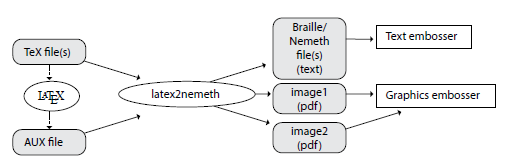
\includegraphics[width=1\linewidth]{images/fig 1.png}
    \caption{The flow of Nemeth files generation.}
\end{figure}

According to the Nemeth code, mathematical expressions with spatial meaning, such as fractions, can be represented in a two-dimensional or in linear, one-dimensional manner.

Our current implementation supports a linear representation, with the exception of array structures and arrays of equations that are represented in a two-dimensional matrix format. In order to correctly indent array structures, they always start the beginning of a new line.

\subsection*{Image Support}

The latex2nemeth tool also provides image support. That is, certain LaTeX graphics macros expressed in the PSTricks graphics library can be filtered so that certain text and mathematics descriptions illustrated in figures are transformed into Braille Nemeth and thus are properly rendered in PDF format so as to be readable by blind persons as properly embossed images and text. An example is given in Figure 2.

\begin{figure*}[h]
    \centering
    
\includegraphics[width=1\textwidth]{images/fig2a.png}
    
\includegraphics[width=0.6\textwidth]{images/fig2b.png}
    \caption{Graphics support example}
\end{figure*}

More specifically, every PSPicture envivonment inside a TeX/LaTeX document, that contains PSTricks images, is filtered so that each mathematical expression, enclosed by the TeX mathematical delimiter, \$, is transformed into Neme\-th/Braille. In the same Figure, the label of the center of the displayed circle, O, is transformed into its corresponding Nemeth/Braille representation, (\fontspec[Script=Braille]{DejaVu Serif}⠠⠕\fontspec{Latin Modern Roman}). Furthermore, each PSTricks picture is rendered as a separate LaTeX source file that can be compiled separately into PDF, so as to be embossed as tactile graphics separately from the Nemeth/Braille text output. Thus, as illustrated in Figure2, more than one image source LaTeX files can be generated from a source LaTeX document that contains more than one PSTricks images. This kind of rendering is compatible with the BANA Guidelines for Tactile Graphics (BANA, 2010). Note that in this way, plain text information can also be rendered, as embedded into mathematics mode.

\section*{IMPLEMENTATION}

The transcriber is based on a parser for the LaTeX language. The language of TeX/LaTeX has two distinct modes: text and mathematics. The parser recognizes most of the most common LaTeX commands and environments in text mode, supporting both English and Greek characters and covers most structures and basic mathematical symbols (see Section 2). The program is developed in the Java programming language using the JavaCC compiler generation tool (Kodaganallur, 2004) for the generation of the parser. The process of LaTeX to Braille transcription is as follows: Each paragraph and each environment in the input LaTeX sources are processed separately. In text mode, each character token is recognized and transcribed into its corresponding Braille symbol by using a certain symbol table. Only numerical expressions are lexically scanned as atomic entities through appropriate regular expressions, eg number 13.455, since, according to Braille code, a certain number sign must precede the whole numerical expression and not every single digit of it. In mathematical mode, both in inline mathematical expressions as well as in mathematical environments, all expressions are parsed, thus creating appropriate syntactical trees. The above process implements the front-end of the mathematical parser, while the back-end is a Nemeth code generator, which complies with (Nemeth, 1972). The abstract syntax trees for mathematics expressions are independent of the TeX/LaTeX language and thus it is easy for the program to be extended so as to implement different back-ends, that is, representations of mathematical expressions different than Nemeth. Given that the tool presented provides abstract representations of mathematical expressions in the above format, implemented as an API in the Java programming language, it can be used as a framework for translating into various forms of appropriate representations for the visually impaired such as audio representations of Mathematical expressions in the form of MathSpeak (Schleppenbach, Said, \& Nemeth, 2007).

 
\begin{figure}[h]
    \centering
    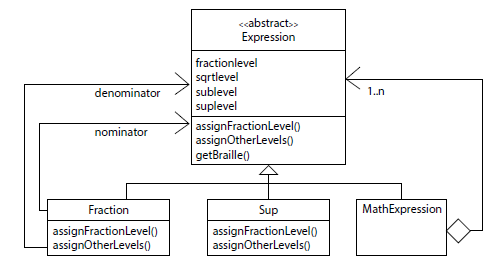
\includegraphics[width=1\linewidth]{images/fig 3.png}
    \caption{Classes of the abstract syntax tree.}
\end{figure}

In Fig. 3 a class diagram showing some of the classes that compose the abstract syntax tree of a mathematical expression is illustrated, as generated internally by the parser. This configuration is a variation of the Interpreter Design Pattern (Gamma, Helm, Johnson, \& Vlissides, 1995). As an example, we take the following expression:

\[e^{{x}^{b+1}} + \frac{1}{1+\frac{1}{x+1}}\]

The above expression is rendered in Nemeth Braille code as 

e<exp>x<exp><exp>b+1<base> \\
<plus> \\
<beginfrac><beginfrac>\\
1\\
<fractionbar>\\
<frac>1<fractionbar>x+1<endfrac>\\
<endfrac>\\

Due to the very limited symbol set available in 6-dot Nemeth encoding, expressions depend on the context witch they appear into, as illustrated in the example above. The inner exponential, with base \textit{x}, is denoted by a double <exp> symbol, while the rendering of the outer exponential, with base \textit{e}, has a single <exp> indication. Correspondingly, the fraction expression is formed recursively by adding a double-fraction (a twice-repeated <beginfrac> symbol) for the outer of the complex fraction.

The generation of expressions in the above manner is supported by the two abstract methods of the Expression class, as illustrated in Fig. 3, namely, assignFractionLevel() and assignOtherLevels(). The first method assigns the nesting level for complex fractions, while the second method assigns the nesting levels for the other types of expressions, namely, square roots, superscripts and subscripts. More specifically, during the construction of each expression of the above types, the levels of nesting are specified. The levels of square root, superscript and subscript are calculated in a top-down fashion, that is, for each of the above expression types, first the level of the containing expression is calculated and then the levels of each corresponding subexpression. In this way, the corresponding level increases with depth, so that an exponential inside an exponential has a level of two, while a simple exponential has a level of one.

Conversely, the level of fractions cannot be determined in this way, according to the Nemeth rules. Rather, in the case of a composite fraction, the outer fraction has a fraction level of one, while a fraction inside has a fraction level of two, etc. In this way, in order to correctly calculate the fraction levels, the calculation is performed bottom-up, starting with the inner expressions, which return their fraction level as a return value of the assignFractionLevel() method.


The tool is available as open source software.\footnote{\url{https://sourceforge.net/projects/latex2nemeth/}}  Thus, everyone can have free access to the software for directly using it without any cost and for modifying it programmatically according to their needs. Furthermore, volunteers can contribute to the extension of the software.

\section*{EVALUATION AND CASE STUDY}

\subsection*{Quantitative Evaluation}

In order to measure the accuracy of the translation of our tool we have conducted a quantitative evaluation of the produced Nemeth output. For the evaluation, we have chosen a sample document from AMSMath LaTeX samples (AMS, n.d.), in particular pages 8 and 13. This sample was selected since it is representative of the kind of mathematics expressions encountered in university mathematics courses at both undergraduate and postgraduate level. The particular sample document comprises expressions of variable size and complexity. Since our aim is to evaluate the production of mathematical expressions generated by latex2nemeth, we have only transcribed the mathematics content of the original sample LaTeX file, removing the textual content. Thus, the sample contained:

\begin{itemize}
    \item  918 characters (counting single characters, symbols, composed characters such as a character with a tilde, and automatically generated characters such as those coming from the LaTeX auxiliary file: references, etc);
    \item  LaTeX structures, such as labels, theorem environments, exponents etc. The sample contained 5 labels, 2 theorem environments, 7 references, 76 subindices, 40 exponents, 1 overline structure, 4 equation environments, 1 equation* environment, 1 cases environment, 3 text-inmath structures, 3 split environments, 1 proof environment, 1 eqref structure, 5 tildes, and 1 fraction structure.
\end{itemize}

The above document, in LaTeX format was translated automatically into Nemeth code using the latex2nemeth software tool. Next, the generated code was translated back into the original mathematical notation by two evaluators. The evaluators were two blind students, the first a student of Mathematics, both with good knowledge of Braille and Nemeth. Both back translations were dictated to a sighted teacher with good knowledge of Braille/Nemeth and Mathematics notation, who did not see the original mathematical document in any stage of the procedure. Next, the mathematics translations were compared with the original mathematical document by the authors of this paper. 

We compared each back transcribed text from the two evaluators with the original text, containing a number of expressions that comprise N=918 different symbols in total. From the above symbols, there were found 12 errors by the first evaluator and 32 errors by the second evaluator, counting multiple errors, or 4 and 5 distinct errors, correspondingly.  

In order to quantify the agreement between the two evaluators we have developed an instrument that is based on Cohen’s kappa (Cohen, 1960), a widely used measure of interrater agreement, as follows: We consider each of the N=918 mathematical characters of the expected output as a different item. For each item, each evaluator assigns one of the M=840 available symbols. Thus, we create an \textit{M} × \textit{M} matrix with each p\textsubscript{ij} element representing the observed probability that a symbol in the mathematical text was identified as \textit{i} by the first evaluator and as \textit{j} by the second evaluator. This probability is calculated by dividing the number of times that a symbol in the mathematical text was identified as \textit{i} by the first evaluator and as \textit{j} by the second evaluator, divided by the total number of symbols, N, in the document. For example, \textit{p}$\cong$$\approx$ expresses the probability that a symbol that was identified as $\cong$ by the first evaluator and as $\approx$ by the second evaluator. The probability of agreement on the specific symbol, $\approxeq$, is expressed as \textit{p}$\cong$$\cong$. 

We calculate the observed probability of agreement among the two evaluators, P\textsubscript{o}, as the sum of probabilities of agreement for each symbol: $P_o = \sum_{i=1}^{M} p_{ii}$. We also calculate the probability, P\textsubscript{e} of agreement by chance, as $P_e = \sum_{i=1}^{m} p_{iA}p_{iB}$ where p\textsubscript{iA}, p\textsubscript{iB} are the total probabilities of choosing symbol \textit{i} by the first and second evaluator, correspondingly. These probabilities are calculated as $P_iA = \sum_{j=1}^{M} p_{ij}$ and $P_iB = \sum_{i=1}^{M} p_{ij}$. Then, Cohen’s kappa coefficient is calculated as \[\kappa = \frac{P_o - P_e}{1 - P_e}\]

Based on the above, the interrater agreement is $\kappa$ = 0.98, which is considerably near the value 1 of absolute agreement. Table 3 summarizes the quantitative results of the evaluation.

\begin{table}[ht]
\caption{Quantitative evaluation summary}
\begin{tabular}{cccc}
\hline
\textbf{Evaluator} & \textbf{Number of errors} & \textbf{Percentage} & \textbf{Number of distinct errors} \\ \hline
1 & 12 & 1.3\% & 4 \\ \hline
2 & 32 & 3.5\% & 5 \\ \hline
\end{tabular}
\end{table}

The error rates identified by the two evaluators were, correspondingly, 1.3 and 3.5 percent (average error 2.4\%). The errors are depicted in Table 4. The first error refers to the rendering of the period symbol (character 256, \fontspec[Script=Braille]{DejaVu Serif}⠲\fontspec{Latin Modern Roman}) as decimal point (character 46, \fontspec[Script=Braille]{DejaVu Serif}⠨\fontspec{Latin Modern Roman}). This error was known to us to be produced by the latex2nemth software, since in its current version the program does not discriminate between the period symbol and the comma symbol. Nevertheless, the first evaluator was able to identify the dot symbol, despite its mistaken translation by the latex2nemeth software. Furthermore, the letter Y is usually orally expressed as “Psi” ($\Psi$) by Greek Mathematicians. Similarly, the letter \textit{W} is usually orally expressed as $\Omega$ (Omega). The mistaken translation of $\phi$ (Greek phi symbol – Unicode 03d5) as $\varphi$ (Greek small letter phi – Unicode 03c6) is due to the optical similarity of the two symbols in the original mathematical form. Next, the rendering of of $\Bar{\partial}u$ as $\partial \Bar{u}$  is due to the oral rendering of the two expressions: the oral expression “partial derivative (bar u)” was perceived and orally dictated as “(partial derivative bar) u”, that is, with a different not by the Nemeth language itself, which is designed to avoid ambiguities (Isaacson \& Michaels, 2015). The checking of the Nemeth output by the authors of this paper confirmed that only one distinct error was produced in the printed Braille/Nemeth representation by the transcription tool itself.

\begin{table}[htb]
\caption{Errors in back translation}
\begin{tabular}{cc}
\hline
\textbf{Original expression} & \textbf{Error expression} \\ \hline
$\Bar{\partial}u$ & $\partial \Bar{u}$ \\ \hline
$W^{B(X)}$ & $\Omega^{B(X)}$ \\ \hline
Y & $\Psi$ \\ \hline
$\phi$ & $\varphi$ \\ \hline
. (period) & . (decimal point) \\ \hline
\end{tabular}
\end{table}

Conclusively, the latex2nemeth software was foDejaVu Serifund to translate TeX mathematics documents with an almost absolute accuracy. Apart from a certain error concerning the period, which we are currently implementing its correct identification and rendering in Braille, a small number of errors also found in the above process were produced by the participants themselves, rather than by the tool under evaluation. 

\subsection*{Case Study}

We have also conducted a case study which involved the transcription of a whole book from LaTeX to Braille/Nemeth format and the study of this book by a student of Mathematics in a Greek University. She was a totally blind female student with excellent performance in Mathematics and fluent in reading in the Braille/Nemeth code. The book is entitled \textit{Real Analysis} by A. Anoussis, V. Felouzis, and A. Tsolomitis and it was written in Greek as a standard course on Mathematical Analysis. The book is available at \url{http://myria.math.aegean.gr/labs/dt/braille/books/real.zip} in Braille format. The student studied a course on Mathematical Analysis using the book as a textbook. After studying the course, we presented a set of questions to the student that form a structured interview to assess the satisfaction of the student from the document analysis. The questions involved understandability, difficulty, correctness, and the overall quality of the generated Braille text.

In her answers to the questionnaire, the student reported that the text produced by latex2nemeth is correct and understandable. Also, she reported that she has not identified any mistakes in the mathematical text. She reported that

\begin{quote}
…now I am on the same level with other students. I feel that I am equal to others while before I felt more inferior… My hands are untied because before I wrote some four hundred pages during a semester so that I feared that I would develop tendonitis.
\end{quote}

Overall, the case study and the interview with the student revealed that the book conversion into Braille is appropriate for a blind mathematics student.

The latex2nemeth program has been systematically used for converting other mathematical books into Braille/Nemeth. Currently, seven whole books in Greek and one book in English have been transcribed from LaTeX. All Greek language books have been used by the student as study material in corresponding courses and she has not reported any problems in reading them and has passed the course examinations with flying colors using the transcribed books as exclusive study materials. We aspire to create an extended repository for Mathematics texts available to blind students. The transcribed books are available in \url{http://myria.math.aegean.gr/labs/dt/braille/index-en.html}.

\section*{CONCLUSION}

In this paper, a new software for generating Braille/Nemeth code for blind persons from LaTeX source documents is presented. Furthermore, certain extensions to the Nemeth code rules and set of symbols are proposed. The software has been found to reliably generate mathematical documents for blind persons. A quantitative evaluation has demonstrated the accuracy of translation of an advanced mathematical text into Nemeth. As mentioned above, the importance of this software lies on two factors:
\begin{itemize}
    \item 	the availability of mathematics documents in post-secondary education mostly in LaTeX format and
    \item 	the importance of the reliable transcription of technical/mathematical documents into Braille format in order to meet their educational role.
\end{itemize}
Of course, our work is not complete. For example, support for other languages (other than Greek and English) is lacking and must be added. The software allows the configuration of both text and mathematical output, so the support of languages other than the above as well as of other mathematics formalisms for the blind is straightforward. But most mathematics symbols, such as the standard TeX math fonts, amsfonts and txfonts, are already supported. Currently, the software is available to the community for free usage and modification. It is also intended to be provided also as a web service. We also aspire to the design and implementation of an interface for facilitating the usage of the transcriber by persons with BLV. As stated earlier, a repository of texts in Mathematics and Science is under development, enhancing the access of visually impaired students to scientific and learning content.

\section*{ACKNOWLEDGEMENT}

The work was partially supported by the Research Unit of the University of the Aegean under grant no. 2625.

\end{large}
\clearpage
\section*{REFERENCES}\par 

\leftskip 0.25in
\parindent -0.25in 

AMS (n.d.). \textit{Sample paper for the amsmath package}. \url{http://mirrors.ctan.org/macros/latex/required/amslatex/math/testmath.pdf}

Archambault, D., Batusic, M., Berger, F., Fitzpatrick, D., Miesenberger, K., Stoeger, B. (2005). The Universal Maths Conversion Library: an attempt to build an open software library to convert mathematical contents in various formats. In C. Stephanidis (Ed.), \textit{Proceedings of 3rd international conference on universal access in human-computer interaction (joint with HCI international 2005)}. Las Vegas, Nevada, USA (July 2005).

BANA (2010). \textit{Guidelines and standards for tactile graphics}. The Braille Authority of Northern America.

Cohen J. (1960). A coefficient of agreement for nominal scales. \textit{Educational and Psychological Measurement}, 20, 37–46.

Duxbury Systems. (n.d.). \textit{Duxbury braille translator for windows}. \url{http://www.duxburysystems.com/}.

Egli, C. (2011). \textit{Liblouis – a universal solution for braille transcription services}. Leipzig: Deutsche Zentralbibliothek für Blinde zu Leipzig (ZDB).

Gamma, E., Helm, R., Johnson, R., \& Vlissides, J. (1995). \textit{Design patterns: Elements of reusable object-oriented software}. Boston, MA, USA: Addison-Wesley Longman Publishing Co., Inc.

Gonzúrová, W., \& Hrabák, P. (2012). Blind friendly LaTeX. In K. Miesenberger, A. Karshmer, P. Penaz, \& W. Zagler (Eds.), Computers helping people with special needs, \textit{Proceedings of International Conference on Computers for Handicapped Persons (ICCHP 2012)}. Lecture Notes in Computer Science, vol 7382 (pp. 138–141). Berlin, Heidelberg: Springer.

Gurari, E. M. (2004). TEX4ht: HTML production. \textit{TUG-boat}, 25(1), 39–47.

Hara, S., Ohtake, N., Higuchi, M., Miyazaki, N., Watanabe, A., Kusunoki, K., \& Sato, H. (2000, January). Mathbraille; a system to transform latex documents into braille. \textit{SIGCAPH Computers and the Physically Handicapped} (66), 17–20.

Isaacson, M.D., \& Michaels, M. (2015). Ambiguity in Speaking Chemistry and other STEM Content: Educational Implications.  \textit{Journal of Science Education for Students with Disabilities}, 18(1), article 2. 

Isaacson, M.D., Schleppenbach, D., \& Lloyd, L. (2010/2011). Increasing STEM Accessibility in Students with Print Disabilities through MathSpeak. \textit{Journal of Science Education for Students with Disabilities}, 14(1), article 2. 

Karshmer, A., Gupta, G., Geiger, S., \& Weaver, C. (1999, Jan). The MAVIS project. \textit{BIT (Behaviour \& Information Technology)}.

Karshmer, A. I., Gupta, G., Pontelli, E., Miesenberger, K., Ammalai, N., Gopal, D., Guo,H.-F. (2004). UMA: a system for universal mathematics accessibility. In \textit{Proceedings of the 6th international ACM SIGACCESS conference on computers and accessibility} (ASSETS’04) (pp. 55–62). New York, NY, USA: ACM.

Kodaganallur, V. (2004). Incorporating language processing into Java applications: a JavaCC tutorial. \textit{IEEE Software, 21}(4), 70–77.

Mackichan. (n.d.). \textit{Scientific WorkPlace}. \url{https://www.mackichan.com/}.

Miesenberger, K., Batusic, M., Heumader, P., \& Stöger, B. (2012). MathinBraille online converter. In K. Miesenberger, A. Karshmer, P. Penaz, \& W. Zagler (Eds.), Computers helping people with special needs, \textit{Proceedings of International Conference on Computers for Handicapped Persons (ICCHP 2012)}. Lecture Notes in Computer Science, vol 7382 (pp. 196–203). Berlin, Heidelberg: Springer.

Nemeth, A. (1972). The \textit{Nemeth braille code for mathematics and science notation: 1972 revision}. American Printing House for the Blind. PEF. (n.d.). The portable embosser format. \url{http://pef-format.org/}.

Schleppenbach, D., Said, J., \& Nemeth, A. (2007, June 14). \textit{Communication system and methods}. Google Patents. Retrieved from \url{https://www.google.com/patents/US20070136334} (US Patent App. 10/579, 377).

W3C. (2003). Mathematical Markup Language (MathML) version 2.0 (second edition). \url{https://www.w3.org/TR/MathML2/}.

\end{document}